% !TeX root = ../thuthesis-example.tex

\chapter{\emph{insertRecords} 写入请求序列化设计与实现}
第 \ref{chap:client-design} 章介绍了客户端对数据的预处理工作,在客户端的预处理结束后,写入请求需要通过 RPC 层序列化为字节流,传输到服务器侧,再反序列化为写入请求被 IoTDB 服务器处理。本章将介绍在新 \emph{insertRecords} 写入机制中,在 RPC 层序列化写入请求时的数据包结构设计与实现。

\section{写入请求序列化的设计目标}
正如 \ref{sec:chap2-sec3} 节中所介绍到的,对写入请求的序列化是一个需要权衡的过程:使用复杂的包结构设计可以让请求序列化得到的字节流很小,通过网络传输的开销比较低,但是序列化与反序列化的开销则很大;使用简单的包结构可以减少序列化与反序列化的开销,但是序列化得到的字节流较大,通过网络传输的开销较高。在设计时,设计者需要把握好压缩率与复杂度的平衡点,以获取综合最优的性能。

在对 \emph{insertRecords} 的写入请求进行序列化时,本文的设计目标如下:
\begin{enumerate}
  \item 相比于目前简单的序列化方案,新的序列化方案需要针对时序数据的特点,对数据进行一定程度的压缩,以减小数据包的体积,降低网络传输延迟;
  \item 数据序列化的资源开销需要可控,对 CPU 资源、内存资源的使用要较为轻量;
  \item 数据序列化设计需要具有可拓展性,以保证未来对序列化方案中增加内容时可以保证兼容性。
\end{enumerate}
针对以上以上的设计目标,本文设计了新的 \emph{insertRecords} 写入请求序列化方案。

\section{写入请求序列化总体设计}
\begin{figure}
  \centering
  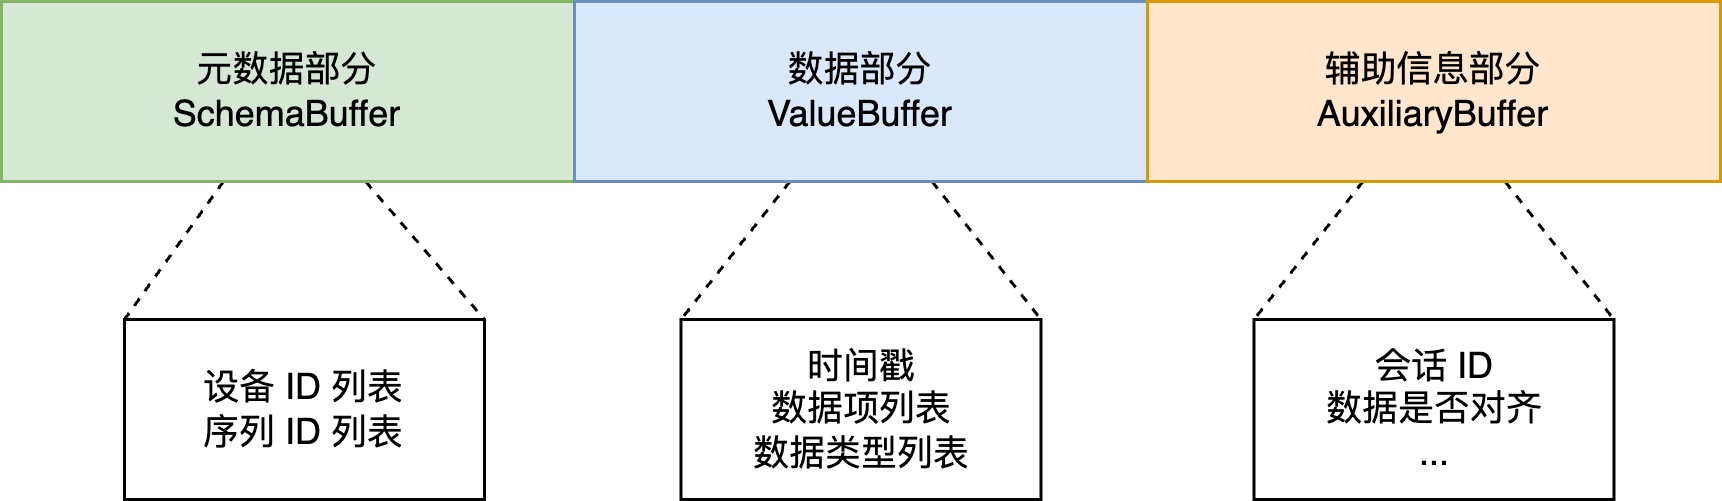
\includegraphics[width=0.9\linewidth]{rpc-general-design.png}
  \caption{写入请求序列化总体设计}
  \label{fig:rpc-general-design}
\end{figure}

在 \ref{sec:chap3-sec2-2-1} 节中,本文介绍了目前 IoTDB 在 Thrift 中对 \emph{insertRecords} 请求的定义。根据各个字段的实际含义,我们可以将它们分成三大部分:元数据部分、数据部分和辅助信息部分。

元数据部分包括设备 ID 和时间序列 ID,它们描述了待写入数据所对应的时间序列都信息。这部分的数据的呈现形式是文本形式,并且其重复度较高,这里的重复度体现在两个方面:
\begin{itemize}
  \item 同一设备或者不同设备的时间序列可能具有相同的 ID,因为它们在现实生活中对应了同样一种类型的实体,例如同样类型的传感器。
  \item 不同设备之间存在部分重复的内容。这是因为 IoTDB 的设备 ID 遵循一种树形的结构,形如 "root.层级1.层级2.层级3"。如果两个设备位于层级树的同一个子树中,那么它们的 ID 中会包含许多相同的部分。
\end{itemize}
针对以上的两个特征,元数据部分非常适合使用字典编码(Dictionary Encoding)进行处理。在本工作的实现中,将元数据部分编码后得到的结果单独保存为一个字节流。

数据部分主要包含时间戳、数值项与数值项的类型。时间戳全都为 8 字节的长整形数据,并且同一个写入请求中不同记录的时间戳可能非常接近;数值项数据可能包含各个类型的数据,如浮点数、整数、字符串等;数据项则都为 1 字节的枚举类型(Enumeration)。数据部分是写入请求序列化后体积最大的部分,对这部分数据进行较为精细化的压缩可以有效减小整个写入请求序列化后的体积。这一部分序列化后的结果也会单独保存为一个字节流。

辅助信息部分主要包括一些标志信息,辅助写入过程中的非核心流程,这部分数据包含会话 ID、数据是否按时间对齐的标志等。这部分数据可能由若干个不同数据类型的标志组成,序列化后的总体积不会很大,因此不需要进行压缩。在未来,\emph{insertRecords} 写入请求中可能会添加更多的辅助信息,因此辅助信息的序列化需要保持一定的拓展性。这一部分序列化后的结果也会单独保存为一个字节流。

下面,本文将分别介绍元数据部分、数据部分和辅助信息部分的序列化设计方案。

\section{写入请求元数据部分序列化与反序列化方案设计}


\section{写入请求数据部分序列化与反序列化方案设计}
对写入请求进行序列化的过程其实本质上是将一份数据转换成字节流,然后传递给下一个处理流程。这个本质与数据存储是类似的,只不过前者将数据交由网络进行传输,而数据存储则将序列化得到的字节流交由磁盘进行存储。因此,我们可以借鉴数据存储领域的一些设计思想。

目前数据库数据存储主要有三种方案:行式存储(Row Storage)、列式存储(Columnar Store)和混合存储(Hybrid Store)。行式存储将一行数据一起保存,相邻的数据项来自不同的列,它们可能类型不同,或者类型相同但是数值的分布不同;列式存储则是将一列数据保存在一起,相邻的数据项不仅类型相同,它们的数值也遵循着共同的分布;混合存储则是将行式存储和列式存储的设计相结合,先将数据按行进行分割成多个块,然后在每个块中按照列的形式存储。行式存储的优势是同一行的数据被聚集在一起,可以方便地访问同一行中的多项数据;列式存储的优势是可以获得更好的压缩比,减少数据体积;混合存储则在一定程度上结合了两者的优势。

同样的,在对写入请求进行序列化时,也可以选择行式存储、列式存储和混合存储。行式存储就是将每一条 Record 的数据一起序列化,列式存储将一条时间序列的数据单独序列化,而混合存储则是先将 Records 分成多批,在每一批内进行列式序列化。

行式序列化的优点在于实现简单,这是因为序列化时一条数据的多个数据项只需要按照顺序逐个转换为字节并添加到字节流中即可,反序列化时也可以按照顺序读取字节流并逐个反序列化单个数据项。但是行式序列化将不同类型的数据全部混合到了一起,导致在压缩时没有办法根据数据的特点进行优化,只能使用通用的压缩算法(如 Snappy\cite{samulowitz2013snappy}、GZip\cite{deutsch1996gzip}、ZSTD\cite{collet2018zstandard} 等)对整体进行压缩,无法实现更加精细化的压缩。

\section{写入请求辅助信息部分序列化与反序列化方案设计}
\section{写入请求序列化与反序列化实现}
\section{本章小结}